\chapter{A rendszer specifikációi és architektúrája}
\label{chap:specifikacio}

A szakdolgozat előző fejezetében bemutatott akusztikai és mélytanulási elméleti alapokra építkezve jelen fejezet a megvalósított hangszerfelismerő rendszer mérnöki és szoftverfejlesztési tervezését ismerteti. Egy gépi tanulási alapú valós idejű hangfelismerő rendszer fejlesztése során nem csupán a neurális hálózat architektúrájára kell fókuszálni, hanem egy olyan robusztus csővezeték (pipeline) kialakítására is, amely képes a nyers adatok betöltésétől kezdve az adatok transzformációján át egészen a végfelhasználói valós idejű interakcióig minden lépést zökkenőmentesen kiszolgálni.

Ez a fejezet definiálja a rendszerrel szemben támasztott funkcionális és nem funkcionális követelményeket, bemutatja a felhasználói eseteket (Use Case), valamint részletezi az alkalmazás belső szoftverarchitektúráját és a technológiai választások hátterét.

\section{Célkitűzések és követelményelemzés}

A fejlesztés fő célkitűzése egy olyan keretrendszer létrehozása volt, amely képes előre felvett zenei adathalmazokon különböző jellemzőkinyerési módszereket alkalmazni, azokkal modern konvolúciós neurális hálózatokat tanítani, majd a legpontosabb modellt egy valós idejű (mikrofonos) környezetben is megbízhatóan futtatni.

\subsection{Funkcionális követelmények}
A funkcionális követelmények azokat a konkrét folyamatokat és szolgáltatásokat írják le, amelyeket a rendszernek feltétlenül nyújtania kell a sikeres működés érdekében:
\begin{itemize}
    \item \textbf{Adathalmazok fúziója és tisztítása:} A szoftvernek képesnek kell lennie nyílt forrású (pl. NSynth, Good-sounds) és saját gyűjtésű adathalmazok egyesítésére, a hibás vagy csendes minták algoritmikus szűrésére.
    \item \textbf{Jellemzőkinyerés (Feature Extraction):} A nyers \texttt{.wav} fájlokból automatikusan generálni kell a spektrogramokat (STFT és Mel-spektrogram) a megadott ablakozási paraméterekkel, és azokat hatékony Numpy mátrix formátumban menteni.
    \item \textbf{Modell tanítása (Training Pipeline):} Egy konfigurálható csővezeték megléte, amely betölti az előkészített adatokat, definiálja a 2D CNN architektúrát, majd korai leállás (early stopping) használatával optimalizálja a modellt, és kimenti a legjobb súlyokat.
    \item \textbf{Valós idejű predikció:} Egy önálló futtatható modul, amely másodpercenként rögzíti a számítógép mikrofonjának jelét, valós időben jellemzőt von ki, és a betanított Keras modellen lefuttatva terminálos felületen jelzi a felismert hangszercsaládot.
\end{itemize}

\subsection{Nem funkcionális követelmények}
A nem funkcionális követelmények a rendszer működésének minőségi mutatóira fókuszálnak:
\begin{itemize}
    \item \textbf{Alacsony késleltetés (Low Latency):} A valós idejű működés kritikus feltétele, hogy az 1 másodperces audio ablak rögzítése és a predikció megjelenítése között eltelt idő ne haladja meg a 200--300 milliszekundumot, ezáltal a felhasználó azonnali visszajelzést kapjon.
    \item \textbf{Erőforrás-hatékonyság:} A jellemzőkinyerésnek és a predikciónak CPU-n is zökkenőmentesen kell futnia, elkerülve a memóriaszivárgást egy végtelenített valós idejű futás (pl. folyamatos élő koncert figyelése) során.
    \item \textbf{Modularitás:} A kódnak lazán csatolt (loosely coupled) szkriptekből kell állnia, hogy a jellemzőkinyerési algoritmus, a neurális háló architektúrája vagy a mikrofonos rögzítési logika egymástól függetlenül módosítható vagy cserélhető legyen.
\end{itemize}

\section{Használati esetek (Use Case modell)}

A rendszer interakciós felületeit és főbb felhasználási forgatókönyveit egy UML Use Case diagram (\ref{fig:usecase}.~ábra) segítségével modelleztük. Két fő aktort azonosíthatunk:
\begin{enumerate}
    \item \textbf{Felhasználó / Kutató:} Az a mérnök vagy adattudós, aki a modell betanításáért és teszteléséért felelős.
    \item \textbf{Mikrofon / Bemenet (Rendszer-aktor):} A valós idejű adatáramlást biztosító hardveres periféria, amely automatikusan triggeli a rendszer predikciós eseményeit.
\end{enumerate}

\begin{figure}[htbp]
    \centering
    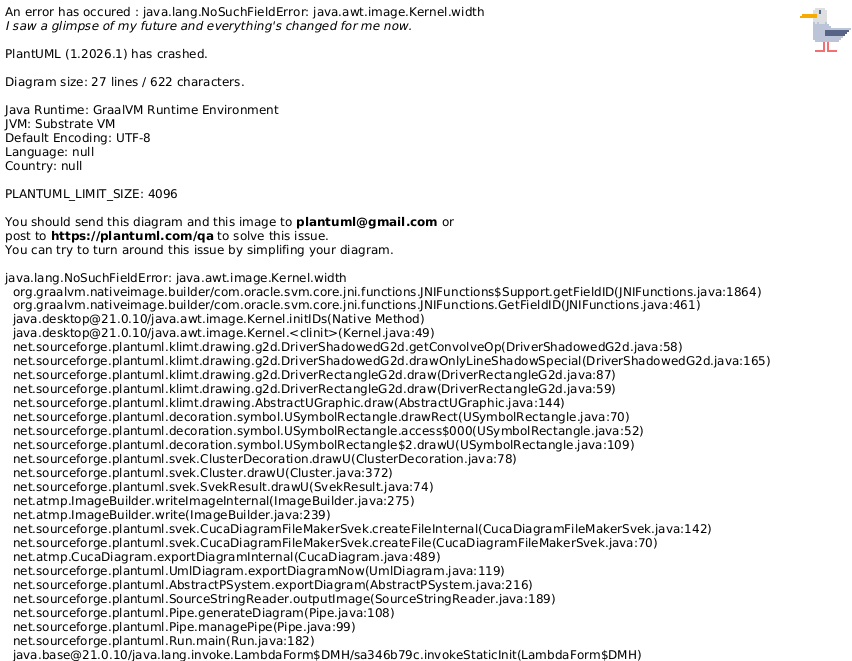
\includegraphics[width=\textwidth,height=0.5\textheight,keepaspectratio]{fig_usecase.png}
    \caption{A hangszerfelismerő rendszer főbb használati esetei (UML Use Case diagram)}
    \label{fig:usecase}
\end{figure}

A használati esetek világosan elkülönítik a "laboratóriumi" vagy kutatási fázist (adatelőkészítés és tanítás) a "produkciós" fázistól (élő predikció). Fontos tervezési szempont volt, hogy a valós idejű hangfelvétel folyamata szorosan inkluzív (\textit{<<include>>}) kapcsolatban álljon a hangszer predikciójával, hiszen a mikrofon bufferének megtelése azonnal és megszakítás nélkül aktiválja az osztályozó modult.

\section{Rendszerarchitektúra és adatfolyam}

Egy robusztus gépi tanulási rendszer architektúrája túlmutat magán a neurális hálózaton; magában foglalja az adatbeviteli (ingestion), az adatfeldolgozási (preprocessing) és az eredmény-megjelenítési (serving) rétegeket is. A megvalósított rendszer szoftverarchitektúráját és az adatok útját a \ref{fig:architecture}.~ábra UML komponensdiagramja vizualizálja.

\begin{figure}[htbp]
    \centering
    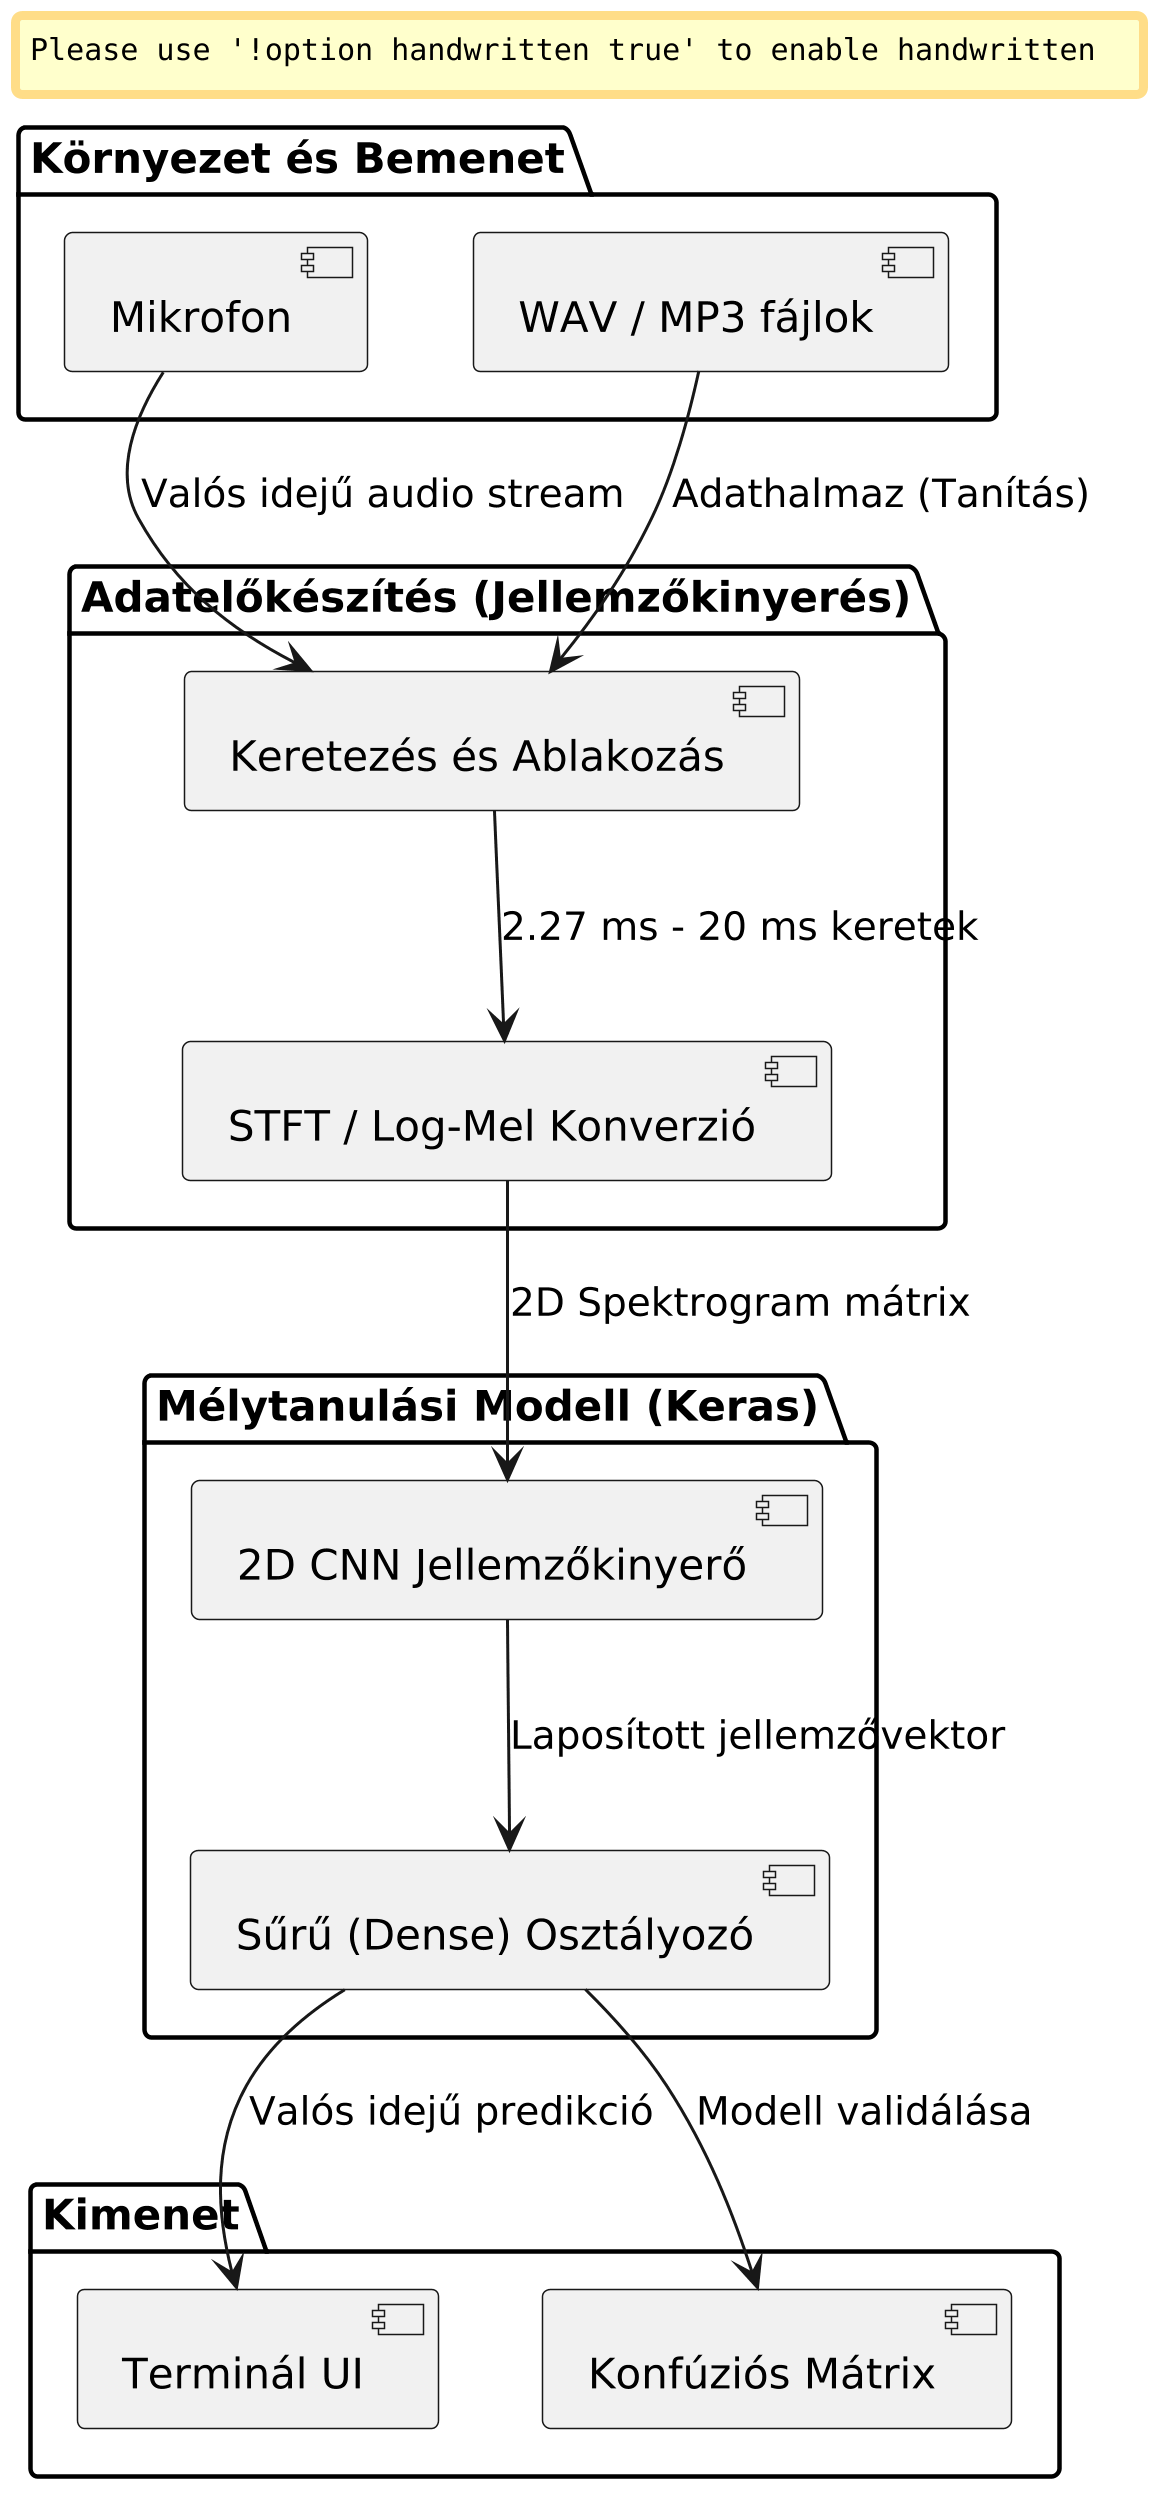
\includegraphics[width=\textwidth,height=0.65\textheight,keepaspectratio]{fig_architecture.png}
    \caption{A rendszerarchitektúra és a folyamatos adatfolyam (UML Komponensdiagram)}
    \label{fig:architecture}
\end{figure}

Az architektúra négy logikailag szeparált csomópontra (csomagra) bontható:
\begin{enumerate}
    \item \textbf{Környezet és Bemenet:} Felelős az adatok biztosításáért. Offline fázisban a \texttt{.wav} és \texttt{.mp3} fájlokból álló hatalmas adathalmazokat biztosítja lemezről, míg online fázisban a rendszer közvetlen I/O kapcsolatot tart a számítógép hangkártyájával.
    \item \textbf{Adatelőkészítés (Jellemzőkinyerés):} Ez a modul a rendszer "szíve" az akusztikai feldolgozás szempontjából. A beérkező folytonos hanghullámokat átfedő keretekre (framing) és ablakokra vágja, majd elvégzi a Fourier-transzformációt (STFT) és a Mel-szűrőbankos konverziót. Kimenete mindig egy fix dimenziójú 2D mátrix, amely már skálázva, normalizálva áll készen a modell számára.
    \item \textbf{Mélytanulási Modell (Keras):} A 2D konvolúciós rétegekből felépülő jellemzőkinyerő, majd az azt követő Sűrű (Dense) osztályozó hálózat. Bemenete a képszerű spektrogram, kimenete pedig egy valószínűségi vektor, amely a hangszer-osztályok eloszlását mutatja.
    \item \textbf{Kimenet:} A fejlesztői terminálon (CLI) megvalósított frissülő felület, amely élőben listázza a predikciós százalékokat, valamint az offline validációs fázisban itt generálódnak a konfúziós mátrixok és a tanulási görbék.
\end{enumerate}

\section{Alkalmazott technológiák és fejlesztői környezet}

A projekt megvalósítása során kiemelt szempont volt a nyílt forráskódú, ipari szabványnak számító eszközök használata, amelyek kiterjedt dokumentációval és tudományos elfogadottsággal rendelkeznek. A fejlesztés Mac OS és Windows operációs rendszereken egyaránt tesztelve lett, biztosítva a platformfüggetlenséget.

\subsection{Programozási nyelv és alapkörnyezet}
A rendszer gerincét a \textbf{Python} programozási nyelv adja. A Python választását annak egyedülálló adattudományi és gépi tanulási ökoszisztémája, valamint a gyors prototipizálást támogató absztrakciói indokolták. A numerikus számításokat, a mátrix-műveleteket és a spektrogramok memóriahatékony tárolását a \textbf{NumPy} könyvtár biztosítja, míg az adatok struktúrált elemzését és tisztítását a \textbf{Pandas} adatkeretek (DataFrames) végzik. A valós idejű, alacsony késleltetésű mikrofonos rögzítést a \textbf{sounddevice} C-alapú Python wrapper hívásai teszik lehetővé.

\subsection{Akusztikai jelfeldolgozás: Librosa}
A hangjelek beolvasásához, csendek levágásához, és a komplex idő-frekvencia transzformációk (STFT, Mel-spektrogram, MFCC) elvégzéséhez a \textbf{Librosa} könyvtárt alkalmaztam. A Librosa a zenei és audio elemzés (MIR) legelismertebb Python eszköze, amely natívan támogatja a pszichoakusztikai skálákat (például a Mel-skálát), így drasztikusan lerövidíti az akusztikai algoritmusok implementációs idejét, garantálva a laboratóriumi pontosságot.

\subsection{Mélytanulási keretrendszer: TensorFlow és Keras}
A mesterséges neurális hálózat architektúrájának definícióját, a modell tanítását és a valós idejű predikciók inferenciáját a \textbf{TensorFlow} platformon futó \textbf{Keras} API végzi. 
A Keras választása a rendkívül gyors fejlesztési ciklus, a kényelmes réteg-absztrakciók (Conv2D, MaxPooling, Dropout) és a könnyű menthetőség miatt történt. A modell betanítása és az adathalmaz validálása nagy kapacitású hardveres környezetben futott, de az inferencia (az élő felismerés) során az elkészült hálózat olyan mértékben optimalizált maradt, hogy egy átlagos számítógép processzorán (CPU) is akadás nélkül, töredékmásodperces válaszidővel képes működni.
